%----------- portada --------------------------------------------------
\newpage
\thispagestyle{empty}
{\pagestyle{empty}\linespread{1}\parindent0pt
\vspace*{0.5cm}

\vfill 

\begin{center}
{\huge \textbf{\introprog}
\par	\vspace{5cm}{\Large \textbf{Andrés Becerra Sandoval}} 
     }

\end{center}

\vfill
\begin{flushright}
{\small
Traducción y Adaptación del libro \\
`'How to think like a computer scientist, learning with Python", \\
escrito por: \\
Allen Downey\\
Jeffrey Elkner\\
Chris Meyers\\
}
\end{flushright}

\vfill



\begin{center}

\includegraphics[scale=0.2]{illustrations/logo/LogoVerticalNegro.eps} 
\end{center}
\begin{center} {\Large Facultad de Ingeniería} \end{center}
\vfill

}
\pagebreak

%----------------------------------------- creditos javeriana--------------------------

\thispagestyle{empty}
\vfill  
\includegraphics[scale=0.2,angle=270]{illustrations/logo/LogoHorizontalNegro.eps} \\
 
\parindent0pt
{\tiny \ }

{\scriptsize 
Rector: Jorge Humberto Peláez, S.J.\\
Vicerrector Académico: Antonio de Roux\\
Vicerrector del Medio Universitario: Gabriel Jaime Pérez, S.J.\\

Facultad de Ingeniería\\
Decano Académico: Jorge Francisco Estela \\
Decana del Medio Universitario: Claudia Lucía Mora \\


Titulo:  \introprog \\
Titulo original: How to think like a computer scientist, learning with Python
Autores: Allen Downey, Jeffrey Elkner, Chris Meyers \\
Traducción y adaptación: Andrés Becerra Sandoval \\
Colección: Libro\\

ISBN: 978-958-8347-22-6 \\

Coordinador Editorial: Ignacio Murgueitio\\
Email: mignacio@javerianacali.edu.co

© Derechos Reservados\\
© Sello Editorial Javeriano\\

Correspondencia, suscripciones y solicitudes de canje:\\
Calle 18 \# 118-250\\
Santiago de Cali, Valle del Cauca\\
Pontificia Universidad Javeriana\\
Facultad de Ingeniería\\
Teléfonos: (57-2) 3218200 Exts. 233 - 518 Fax 555 2823\\
Email: abecerra@javerianacali.edu.co \\

Formato 17  x  25 cms\\
% Diseño e Impresión: Multimedios PUJ Cali\\

Diseño de Carátula: 
Patricia Mejía, basada en una imagen de Ken Manheimer \\
http://myriadicity.net

Impresión: 2009
}
%-------------------copyright--------------------------------------------------
\newpage
\thispagestyle{empty}
\vspace{0.25in}

Se concede permiso para copiar, distribuir, y/o modificar este documento bajo
los terminos de la GNU Free Documentation License, Versión 1.1 o cualquier
versión posterior publicada por la Free Software Foundation; manteniendo 
sin variaciones las secciones ``Prólogo,'' ``Prefacio,'' y ``Lista de contribuidores,''
sin texto de cubierta, y sin texto de contracubierta. Una copia de la licencia
está incluida en el apéndice titulado ``GNU Free Documentation License'' y una 
traducción de ésta al español en el apéndice titulado ``Licencia de Documentación Libre de GNU''.

La GNU Free Documentation License también está disponible a través de \url{www.gnu.org}
o escribiendo a la Free Software Foundation, Inc., 59 Temple Place,
Suite 330, Boston, MA 02111-1307, USA.

La forma original de este libro es código fuente \LaTeX\  y compilarlo
tiene el efecto de generar un libro de texto en una 
repesentacion independiente del dispositivo que puede ser convertida a otros 
formatos e imprimirse.

El código  fuente \LaTeX\  para este libro y mas información sobre este proyecto
se encuentra en los sitios web:

\begin{verbatim}
      http://cic.javerianacali.edu.co/~abecerra
      https://github.com/abecerra/thinkcs-py_es
      http://www.thinkpython.com
\end{verbatim}

Este libro ha sido preparado utilizando \LaTeX\ y las figuras
se han realizado con xfig.  Todos estos son programas de código
abierto, gratuito.

\vspace{0.25in}
%------informacion bibliografica -----------------------------------------------------------
\newpage
\thispagestyle{empty}

\begin{center}
\framebox{
  \begin{minipage}{11cm}
   \footnotesize 
    Downey, Allen \\
    Introducción a la programación con Python / Allen Downey, Jeffrey Elkner, Chris Meyers; 
    traducido y adaptado por Andrés Becerra Sandoval. – Santiago de Cali: Pontificia Universidad Javeriana, 
    Sello Editorial Javeriano, 2009. \\
    305 p. ; 26 cm.  \\ \\
      
    Incluye referencias bibliográficas e índice. \\ \\
       
    ISBN  978-958-8347-22-6\\ \\
     
    1. Programación (computadores electrónicos) -- Metodología 2. Python (lenguaje de programación 
    para computadores) I. Meyer, Chris II. Pontificia Universidad Javeriana (Cali) III. How to think 
    like a computer scientist: learning with python IV. Tít. \\ \\

    SCDD 005.1	\hfill						   BPUJC

   \end{minipage}
   }
\end{center}